\chapter{Analisi}
%I suggest referencing stuff as follows: \cref{fig:random-image} or \Cref{fig:random-image}
%\begin{figure}
%	\centering
%	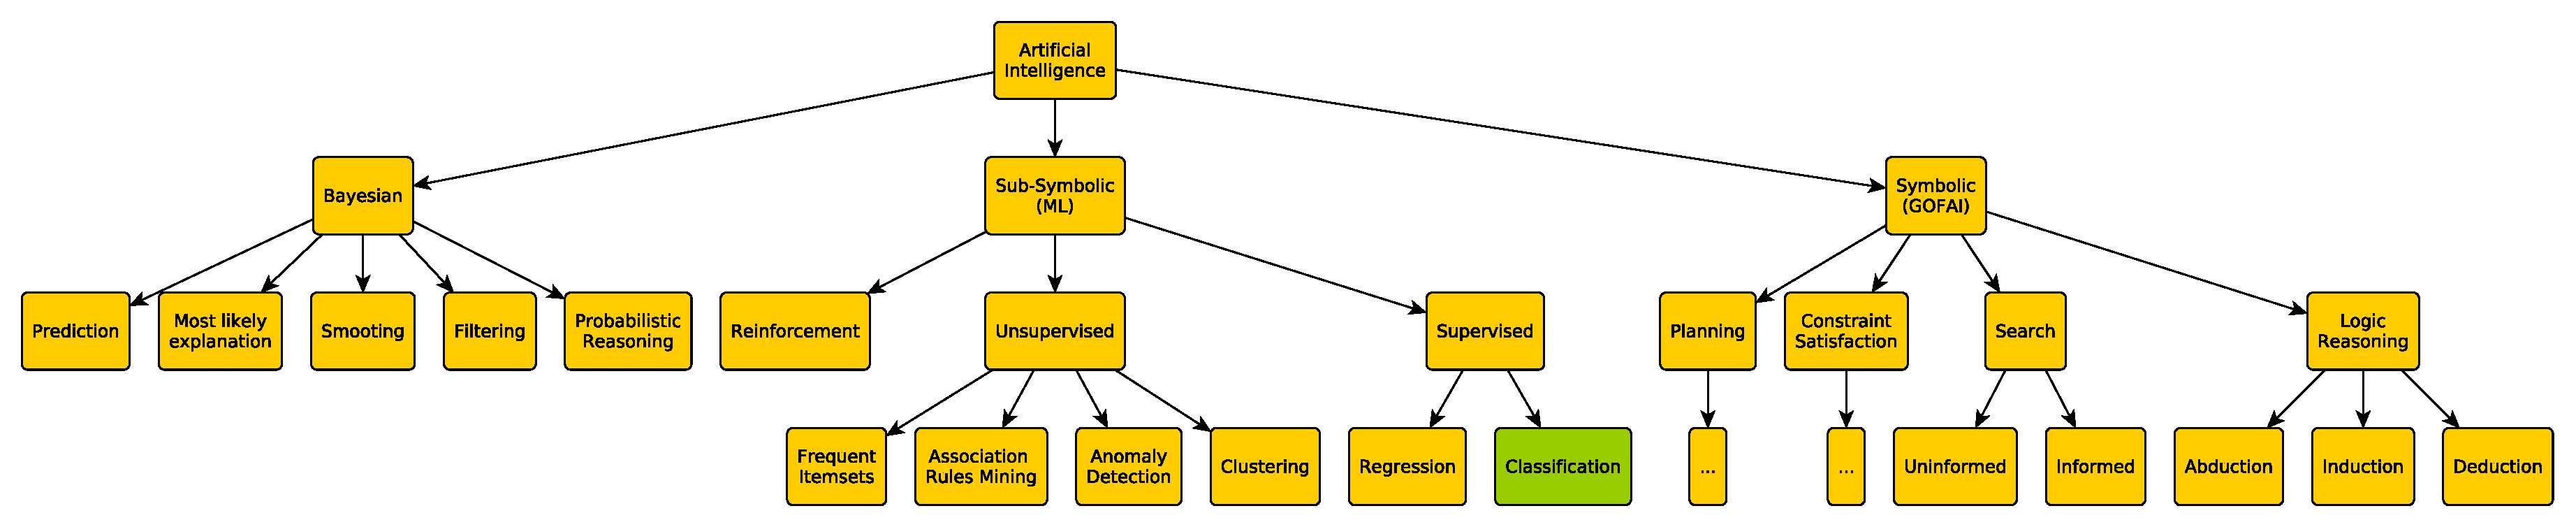
\includegraphics[width=.8\linewidth]{figures/random-image.pdf}
	%\caption{Some random image}
	%\label{fig:random-image}
%\end{figure}

\section{Requisiti}

Lo scopo principale del progetto è la realizzazione di una interfaccia web (quindi interpretabile da un qualsiasi browser moderno) che permetta l'interazione con il sistema software di simulazione
\textit{Alchemist} in modo intuitivo e \textit{user-friendly}. Il compito dell'applicativo sarà quindi quello di comunicare, attraverso apposite \ac{API}, con l'infrastruttura server preesistente e presentare in seguito a cambiamenti della simulazione in corso o a richieste da parte dell'utente, un'interfaccia grafica che ne rappresenti i risultati.
\subsection{Requisiti funzionali}
\begin{itemize}
	\item L'applicativo dovrà presentare un interfaccia grafica all'interno di un web browser.
	\item In una tipica simulazione di \textit{Alchemist} (come discusso nel paragrafo) sono presenti dei nodi. L'applicativo quindi dovrà essere in grado di rappresentare in un piano bidimensionale la posizione di tali nodi all'interno di un contesto grafico. Ciò implica ovviamente che con l'evolversi della simulazione il contesto grafico debba essere aggiornato. \footnote{Date le diverse \textit{incarnation} e i diversi possibili scenari che \textit{Alchemist} può modellare non è detto che i nodi cambino di posizione.}
	\item Ogni nodo contiene diverse proprietà, reazioni, concentrazioni etc. L'interfaccia dovrà permettere di ispezionare il contento di ciascun nodo. 
	\item L'interfaccia dovrà controllare lo stato attuale della simulazione. Ciò vuol dire poterla eseguire o mettere in pausa.
\end{itemize}

\subsection{Requisiti non funzionali}
\begin{itemize}
	\item Interagendo con l'interfaccia, non si devono verificare tempi di risposta eccessivi. Per esempio se l'utente decide di ispezionare un nodo, il recupero di tali informazioni deve essere presentato in tempi ragionevoli.
	\item  La comunicazione con l'infrastruttura server non deve impattare in modo negativo l'utilizzo dell'interfaccia stessa. 
	\item L'architettura delle componenti grafiche deve essere estendibile e facilmente 
\end{itemize}

\section{Analisi dei requisiti}

\section{Vincoli}

\section{Analisi e Modello del Dominio}
